\documentclass[12pt]{scrartcl}
\usepackage[utf8]{inputenc}
\usepackage[english,croatian]{babel} % neki citati su na izvornom engleskom, ali hrvatski je naravno glavni jezik eseja
\usepackage[unicode]{hyperref}
\usepackage{amsmath,amssymb,amsthm}
\usepackage{mathtools}
\usepackage{thmtools}
\usepackage{csquotes}
\usepackage{xcolor}
\usepackage[backend=biber]{biblatex}
\hypersetup{
    colorlinks,
    linkcolor={red!50!black},
    citecolor={blue!50!black},
    urlcolor={blue!80!black}
}

\addbibresource{literatura.bib}
\MakeOuterQuote{"}
\declaretheorem{teorem}
\declaretheorem[style=definition,sibling=teorem,qed=$\vartriangleleft$]{definicija}
\declaretheorem[name=Primjer,style=definition]{example}

\newcommand{\T}{^\mathsf T}
\newcommand{\mat}[1]{%
    \ifmmode%
        \mathbf{#1}%
    \else%
        $\mathbf{#1}$%
    \fi%
}
\newcommand{\vek}[1]{\mat{#1}}
\newcommand{\citat}[2]{\begin{quotation}\textit{#1}\end{quotation}\begin{flushright}---#2\end{flushright}}
\newcommand{\primjer}[2]{%
    \renewcommand\qedsymbol{$\vartriangleleft$}%
    \begin{example}%
        #1%
    \end{example}%
    \begin{proof}[Rješenje]%
        #2%
    \end{proof}%
    \renewcommand\qedsymbol{$\Square$}
}

\author{Mauro Raguzin}
\title{Korijen --- 1 algoritam, 3 implementacije}
\date{\today}

\begin{document}
\maketitle
\tableofcontents
\pagebreak

\section{Uvod}
%V1:Ovaj esej se bavi naoko jednostavnim i elementarnim numeričkim algoritmom: računom kvadratnog korijena. Iako u osnovi poznat tisućama godina,
%ovaj algoritam ima fascinantan broj varijacija, što u njegovoj osnovnoj konceptualizaciji neovisnoj o namijenjenom izvršitelju, što u konkretnim
%formama koje dobiva u ovisnosti o različitim računalnim arhitekturama na kojima se povijesno implementirao.
Izračunati kvadratni korijen realnog broja --- koliko bi to moglo biti teško? Iako u osnovi poznat tisućama godina,
ovaj algoritam ima fascinantan broj varijacija, što u njegovoj osnovnoj konceptualizaciji neovisnoj o namijenjenom izvršitelju, što u konkretnim
formama koje dobiva u ovisnosti o različitim računalnim arhitekturama na kojima se povijesno implementirao.

U ovom eseju obrađujemo u detalje ovaj algoritam kroz povijest, od nekoliko stoljeća prije Krista
do današnjeg kompjutoriziranog doba u kojem su precizne i vrlo efikasne varijante
ovog algoritma od presudne važnosti u raznolikim poljima primjene, poput simulacije, digitalne fizike i računalne grafike. Usput ćemo predstaviti
i neke analize posebno zanimljivih modernih računalnih implementacija te predstaviti mjerenja obavljena na današnjim računalima za različite implementacije.
% TODO: zašto baš tri implementacije? Navedi tu ukratko razlog + koliko smo ih ustvari točno obradili!

\section{Povijest računa kvadratnog korijena}\label{sec:hist}
    \citat{\begin{otherlanguage}{english}
        Seeing there is nothing that is so troublesome to Mathematicall practise, nor that doth more molest and hinder Calculators,
    then the Multiplications, Diuisions, square and cubical Extractions of great numbers, which besided the tedious expence
    of time, are for the most part subiect to many slippery errors. I began therefore to consider in my minde, by what certaine
    and ready Art I might remoue those hindrances~\cite[str.~194]{taocp2}.
    \end{otherlanguage}}{John Napier (1616.)}

\subsection{Babilonski period}

Najstariji poznati zapisi netrivijalnih numeričkih algoritama "u akciji" potiču iz drevnog Babilona --- poznato
 je da su babilonski matematičari znali računati zbroj, razliku, umnožak, recipročnu vrijednost te kvadratni korijen brojeva prikazanih
u \emph{seksagezimalnom} (baza $60$) brojevnom sustavu; potonje dvije stavke su pak mogli računati svojevrsnom linearnom interpolacijom iz
sastavljenih tablica, ili preciznije, ploča. Naime, ekskavirane su razne ploče s korespondencijom između brojeva $n$ i $n^2$. Korektne ploče s
recipročnim vrijednostima brojeva su pronađene samo za "regularne" brojeve do određene duljine, tj.\ one s konačnim prikazom u seksagezimalnom sustavu, jer
se čini da Babilonjani nisu poznavali ponavljajuće nizove znamenki~\cite{KnuthBabylon}.

Valja napomenuti da je starobabilonski brojevni sustav
također podrazumijevao rad u jednoj vrsti "pomičnog zareza" koja se temelji na činjenici da bilo koji zapisan broj može odjednom predstaviti
\emph{bilo koji} svoj umnožak sa $60^k,\,k\in\mathbb{Z}$. Iako nam ovakav "nedeterminizam" danas može zvučati suviše složenim i svakako
neprikladnim za računalnu implementaciju, bio je ključan za relativno precizne rezultate do kakvih su starobabilonski matematičari redovito
dolazili, koristeći pritom donekle intuitivno očekivanje koliko bi brojevi trebali biti veliki ili mali u kontekstu u kojem se zadani račun rješava
(tipično je to bilo u sklopu nekog računa iz stvarnosti, sa zadanim jedinicama i očekivanim redom veličine dimenzija rezultata) kako bi mogli odrediti
prikladan faktor skaliranja u svakom međukoraku računa. Ovo znači da su svi aritmetički algoritmi iz tog doba radili podjednako dobro i za 
"realne" i za cijele brojeve, jer bi za praktičnu razliku između njih bila odgovorna osoba koja računa.

Zanimljivo je napomenuti da su pronađeni mnogi spisi koji potječu od oko 2.~stoljeća prije Krista u kojima
se rješavaju zadaci poput izračunavanja dimenzija cisterni sa zadanim ograničenjima, što je dovelo do impresivnih zapisa (koji podsjećaju
na današnje pseudokod-programe!) ručnog izvršavanja
 \emph{algoritama} za rješavanje linearnih, ali i složenijih sustava jednadžbi poput $x+y=a,\ x^2+y^2=b$, za što je očito bilo potrebno
imati ili algoritam za račun korijena ili odgovarajuću tablicu. Primjerice, Babilonjani su aproksimirali $\sqrt 2$ ($N=2$) na ovaj način (prevedeno
u dekadske razlomke)\cite{fowler1998}:
\begin{equation}\label{eq:babiter}
    \sqrt 2 = \sqrt{\left(\frac32\right)^2 - \frac14}\approx\frac32 - \frac12\times\frac14\times\frac23 = \frac32 - \frac{1}{12} = \frac{17}{12}\text.
\end{equation}
Račun započinje uzimanjem početne aproksimacije korijena, $a=\frac32$ u \eqref{eq:babiter}, te uz pretpostavku da je ona veća od prave vrijednosti,
dodavanjem ostatka $B$ koji nam nije poznat, ali za kojeg znamo da mora biti manji od kvadrata početne aproksimacije. Modernim algebarskim riječnikom,
ovo odgovara
\[
    B=a^2-N,
\]
gdje odmah vidimo da ovo povlači $a-B+N<N$, što znači da smo sada dobili aproksimaciju koja je manja od prave vrijednosti. Pritom imamo dualnu situaciju
ako počnemo od manje aproksimacije; slika \ref{sl:babiter} prikazuje najvjerojatniji način na koji su Babilonjani konstruirali i koristili ovaj postupak.
%TODO: slika ovdje, sa stranice 6 citiranog članka; prepiši u TikZ i prilagodi tekst!

Dakako, opisan bi račun, radi dobivanja veće preciznosti rezultata, trebalo iterirati,
uzimanjem dobivene ($\frac{17}{12}$ u \eqref{eq:babiter}) bolje aproksimacije umjesto prethodne
($\frac32$) za nastavak računa, no zapisi s takvim postupcima nisu pronađeni,
vjerojatno zbog toga što se rijetko kada dobije "regularan" međurezultat te zbog toga što
bi potreban račun bio suviše složen, uključujući množenja za koja nisu postojali podaci u dostupnim tablicama za množenje. Stoga se čini da su 
Babilonjani bili uglavnom zadovoljni rezultatom jedne jedine iteracije ove osnovne metode, koja je u biti ekvivalentna mnogo kasnije zabilježenom Herodovom
metodom za račun korijena, potrebnom za evaluaciju poznate Heronove formule za površinu trokuta
\begin{equation*}
    P_{\triangle} = \sqrt{s(s-a)(s-b)(s-c)}\text.
\end{equation*}
Naime, iz originalnog Heronova opisa riječima, prevodeći opet u modernu algebarsku notaciju, dobivamo formulu $\frac12(a+N/a)$, koja je
zaista ekvivalentna $a+\frac12(N-a^2)/a$, iz gornjeg opisa iteracije Babilonjana. Ipak, svakako je računski bilo puno složenije izračunati
$(N-a^2)/a$ od $N/a$. % TODO: spomenuti jako blisku vezu s kasnijom Newtonovom metodom!
Dakle, račun korijena od $N$ se u oba slučaja svodi na rješavanje rekurzivne relacije
\begin{equation}
    a_{n+1}=\frac12\left(a_n+\frac{N}{a_n}\right),
\end{equation}
s prikladnom početnom aproksimacijom $a_0$.

\subsection{Indijski doprinos}
Negdje u prvim stoljećima nakon Krista, danas nepoznati indijski matematičari izumili su dekadski brojevni sustav. Za razliku od svih prijašnjih brojevnih sustava,
uključujući i neke pokušaje pozicionalnih (babilonski, majanski\ldots), ovaj sustav se odlikuje dodjelom težina svakoj brojevnoj poziciji u geometrijski
rastućem poretku te uključuje $0$ kao broj. Lakoća korištenja ovog sustava za svakodnevno računanje je bila ključna za razvoj, po prvi puta
u povijesti, cijelog niza
efikasnih aritmetičkih algoritama za ručno, ali i (puno kasnije) strojno računanje. Među njima se našao i algoritam za kvadratni korijen, brži od onoga
iz starobabilonskog doba, otkriven kao dio tzv.\ Bakhshali rukopisa\footnote{Ovaj rukopis je imenovan po selu u kojem je pronađen krajem 19.\ stoljeća.
Osim algoritma za korijen, sadrži i razne primjere rješavanja diofantskih jednadžbi, kvadratnih jednadžbi te aritmetičkih nizova.},
najvjerojatnije iz 7.\ stoljeća nakon Krista~\cite{bakhshali}.

\begin{figure}
    \caption{Fragment Bakhshali rukopisa~\cite{bakhshali}.}
    \center
    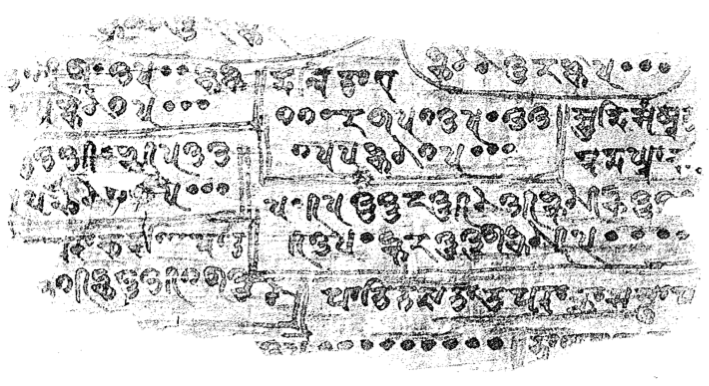
\includegraphics[scale=0.5]{bakhshali}
\end{figure}

U modernoj notaciji, algoritam kaže da za izračunati kvadratni korijen broja $q$ treba krenuti s aproksimacijom $x_0$ i zatim izračunati,
za $n\geq 0$,
\begin{align}
    a_n\: &=\: \frac{q-x^2_n}{2x_n}\\
    x_{n+1}\: &=\:x_n + a_n - \frac{a^2_n}{2(x_n + a_n)}\text.%\\
    %q\: &=\:x^2_{n+1} - \left[\frac{a^2_n}{2(x_n + a_n)}\right]^2\text.
\end{align}

Slično kao i u starobabilonskom slučaju, nema nikakvih indikacija da su staroindijski matematičari ikada iterirali gornje formule više od jedanput.
No, upravo u iteraciji leži najveća moć ove indijske metode --- algoritam kvartično konvergira\footnote{Svaka iteracija
učetverostručuje broj točnih značajnih znamenki,
pod uvjetom da nam je realna računalna aritmetika dovoljno precizna ili da radimo u racionalnoj aritmetici proizvoljne preciznosti.
Za usporedbu, poznata Newton-Raphsonova iteracijska shema konvergira kvadratno.}! Nijedan algoritam
slične efikasnosti nije bio poznat u Europi sve do 18.\ stoljeća.

% \begin{teorem}
%     Bakhshali algoritam za račun kvadratnog korijena kvartično konvergira.
% \end{teorem}
% \begin{proof}
    
% \end{proof}

\section{Moderniji pristupi}
\citat{\begin{otherlanguage}{english}
    Steve Russell certainly didn't know that his Spacewar was using a symplectic integrator.
That term wasn't invented until years later. It is serendipity that the shortest machine language program has the best numerical properties.
\end{otherlanguage}}
{Cleve Moler~\cite{spacewar}}

U ovom odjeljku ćemo razmatrati neke novije pristupe računu korijena, pri čemu mislimo uglavnom na algoritme prilagođene
izvršavanju na digitalnim računalima. Umjesto iscrpnog povijesnog pregleda svih varijanti implementiranih algoritama, usredotočit ćemo se na
nekolicinu \textsl{sui generis} algoritama i njihovih implementacija, analizirajući
njihova numerička svojstva i uspoređujući ih s onima iz odjeljka~\ref{sec:hist}.

\subsection{Algoritam s dvije varijable}
Potreba za računom kvadratnog korijena javila se vrlo rano u povijesti digitalnih računala i odgovarajuće rutine u strojnom jeziku
su ubrzo bile implementirane za računala poput EDSAC-a početkom 1950-ih godina~\cite{gower}. Takva računala tipično nisu imala ugrađen
hardver za brzu aritmetiku s pomičnim zarezom niti su podržavala instrukciju dijeljenja, pa su se tražile metode koje mogu u potpunosti
izbjeći dijeljenje i po mogućnosti koristiti samo operacije zbrajanja te bitnovnog posmaka.

Jedna takva rana metoda dolazi od ekipe predvođene Wilkesom\footnote{TODO} sa sveučilišta u Cambridgeu odgovorne za EDSAC,
inače prvo računalo s pohranjivanjem programa~\cite[str.~32]{ribaric}. Metoda je iterativna i koristi \emph{dvije} varijable te 
u potpunosti zadovoljava spomenute specifikacije. To uspijeva zahvaljujući nekim osnovnim rezultatima koje ćemo sada izvesti za
malo općenitiji slučaj izračunavanja $y/x^{1/n},\,n\in\mathbb{N}$, gdje pretpostavljamo da nas zanimaju samo pozitivni cjelobrojni rezultati, pa
je riječ o funkciji s domenom u $\mathbb{N}^2$ i kodomenom u $\mathbb N$\footnote{Ovo se može interpretirati kao račun u aritmetici
s \emph{fiksnim} zarezom, uz odgovarajuća skaliranja na početku i kraju, što je bilo uobičajeno za rana računala. Pritom želimo da algoritam
računa rezultat do na točnost $2^{-(w-1)}$, gdje je $w$ duljina riječi u bitovima, jer tako osiguravamo točan rezultat u smislu aritmetike
s fiksnim zarezom.}.

Promotrimo dvostruko iterativni proces u varijablama $a_k$ i $c_k$:
\begin{align}
        a_{k+1} &= a_k(1 + \alpha c_k)\label{eq:iter1}\\
        (y^n / x)(1 + c_{k+1}) &= a^n_{k+1}\label{eq:iter2}\text.
\end{align}
Ako $c_k\to 0$ za $k\to\infty$, onda očito vrijedi $a_k\to y/x^{1/n}$ te iz \eqref{eq:iter1} i \eqref{eq:iter2} lako izvodimo
\begin{equation}
    c_{k+1} = (1+c_k)(1+\alpha c_k)^n - 1\text.
\end{equation}
Bitno je da osiguramo konvergenciju; može se pokazati da ako $y^2<x<1$ (skalirano), za $|c_k|<1$ negativan imamo
\begin{equation}\label{eq:edsacscale}
    -1\leq c_{k+1}\leq(1+c_k)e^{-c_k}-1<0\text.
\end{equation}
Odabirom $\alpha=-1/n$ dobivamo kvadratnu konvergenciju ovog sustava~\cite{gower}.

Uvrštavanjem u \eqref{eq:iter1} i \eqref{eq:iter2}, dobivamo:
\begin{align}
    a_{k+1} &= a_k(1-c_k/n)\\
    c_{k+1} &= (1+c_k)(1-c_k/n)^n - 1\text.
\end{align}
Sada općenito vidimo da iz \eqref{eq:edsacscale} slijedi
da su sve vrijednosti niza $c_k$ negativne te da taj niz konvergira ka $0$. Iz \eqref{eq:iter2} pak dobivamo
$|a_k|^n<|y^n/x|$, iz čega možemo zaključiti da je $|a_k|<1$ (skalirano) čim je konačan rezultat isto takav.

Za dobiti formule specifično za račun kvadratnog korijena od $x$, odabiremo $a_0=y=x$ i $c_0=x-1$ te $n=2$, što nam daje:
\begin{equation}
    \begin{aligned}\label{eq:sqrtedsac}
        a_{k+1} &= a_k\left(1-\frac12 c_k\right)\\
        c_{k+1} &= \frac14 c^2_k(c_k-3)\text.
    \end{aligned}
\end{equation}
U ovom posebnom slučaju se konvergencija $a_k\to\sqrt x$ može lako provjeriti direktno po definiciji konvergencije
niza koji je monotono padajući (unutar legalnog raspona $x$-a vrijedi da su sve $c_k$ vrijednosti negativne te rastu tj.
apsolutna vrijednost niza pada) koristeći gornje rezultate o omeđenosti međurezultata; no, uočimo da to možemo pokazati
samo za $0\leq x<3$ po gornjem odabiru početnih uvjeta --- to je jedini raspon unutar kojeg je ova metoda primjenjiva (što se tiče korijena).

Ne samo da ova metoda ima relativno malu stvarnu domenu primjene, ona se također radi preciznosti često mora ograničiti još i više.
Vidimo da je iteriranje sustava \eqref{eq:sqrtedsac} moguće korištenjem množenja, dijeljenja s potencijama od $2$ te zbrajanja i oduzimanja, što
je lako za implementirati na svim procesorima. Ipak, ova metoda, zbog korištenja dvije iteracijske varijable, može akumulirati greške za razliku
od starobabilonske metode. Konvergencija za račun korijena ovom metodom se usporava što je $x$ manji, što znači da bi trebali pred-skalirati argument
što je više moguće (do gornje granice duljine riječi), obaviti račun i na kraju skalirati natrag; štoviše, nužno je
skalirati argument tako da vrijedi $0<x<1$ (skalirano) radi osiguravanja da će konačan rezultat biti $<1$ (skalirano), čime dobivamo
traženu garanciju strojne (u smislu fiksnog zareza) preciznosti. 
Faktor skaliranja bi trebao biti parna potencija od $2$,
kako bi račun korijena bez gubitka prepolovio eksponent.

Iz svega navedenog možemo uočiti da je područje konvergencije ovog algoritma, pogotovo za nama najzanimljiviji slučaj $n=2$, izrazito usko
(u tom slučaju vidimo da je riječ o podskupu od $\{x\mid x\in\left[0,3\right\rangle\}$ za kojeg jedino i možemo primijeniti ovaj algoritam), pa je
zaista bitno primijeniti dosta pred- i post-procesiranja kako bi se izvuklo maksimalno preciznosti iz ovog algoritma.
Gower u \cite{gower} preporučuje raspon ciljni $(\frac12)^n\leq x<1$.
Za računala za koja je
ovaj algoritam bio
namijenjen, to je bila i jedina moguća relativno efikasna opcija.

\subsection{Algoritam bit-po-bit}
Sada ćemo proučiti jednu široko poznatu i implementiranu metodu za račun kvadratnog korijena, najčešće opet domene i kodomene u
$\mathbb{N}$, iako se često koristi s odgovarajućim skaliranjem i za "realne" brojeve
 na platformama gdje je moguća jedino aritmetika s fiksnim zarezom; mi ćemo podrazumijevati da radimo samo nad $\mathbb N$, pa ustvari
 dajemo algoritam za račun $\lfloor\sqrt x\rfloor$.

Riječ je o metodi kojom ljudi mogu dosta efikasno na papiru izračunati korijen, iako je sporija od svih prije obrađenih zbog toga
što u svakoj iteraciji daje samo jednu novu znamenku rezultata. Ipak, popularna je i dandanas upravo zbog svoje jednostavnosti te je
poznato da su neki rani ručni kalkulatori, poput Napierovih kosti (17.\ st.), koristili ovu metodu.
 Opisat ćemo je primjerom
u dekadskom brojevnom sustavu, a nakon toga formalizirati točan postupak za nama zanimljiv binarni sustav.

\primjer{Izračunati $\sqrt{891}$.}
{Kako smo u dekadskom sustavu, znamo da troznamenkasti brojevi mogu imati najviše dvoznamekasti korijen; općenito, $k$-znamenkasti broj
može imati najviše $\lceil\\frac{k}{2}\rceil$-znamenkasti korijen. Mi u biti želimo "riješiti jednadžbu" $(10x+y)^2+z=891$, gdje je 
"ostatak" $z$ potreban jer očekujemo da nam argument neće biti savršeni kvadrat. U tu svrhu krećemo od najznačajnije znamenke rješenja
$x$ --- koja je najveća znamenka koja, kvadrirana i pomnožena sa $100$, daje broj manji ili jednak $891$? Nalazimo da je to $x=2$, pa
uvrstimo to u jednadžbu i tražimo dalje $y$. Budući smo razriješili najznačajniji dio rezultata, možemo oduzeti dobiveni $400$ od $891$,
dobiti $40y+y^2=419$
i nastaviti pretragu kao prije. Tako nalazimo $y=8$ i, kako uvrštavanje u jednadžbu ne daje točno $419$,
znamo da imamo "ostatak" $z>0$. No, nama on nije bitan, pa budući da ustvari računamo $\lfloor\sqrt{891}\rfloor$,
 dovoljno je vratiti naš dobiveni rezultat kao konačno rješenje.}

Općenito, ovaj algoritam se svodi na iterativno traženje najvećeg jednozamenkastog
broja koji zadovoljava da mu je izračunata vrijednost preostalog dijela binomne jednadžbe manja ili jednaka (preostalom) argumentu, sve
dok odredimo vrijednosti svih nepoznanica.

Formalno, imamo zadan $N\in\mathbb N$ i tražimo znamenke $a_1,\dotsc a_n$ ($a_0$ je \emph{najznačajnija}; $a_i$-jevi 
dakako uključuju i odgovarajuću potenciju baze $B$) tako da vrijedi 
\begin{equation}
    N=\left(\sum^n_{i=1}a_i\right)^2+z=N,
\end{equation}
gdje je $n=\lfloor \frac{\log_B N + 1}{2}\rfloor$.
Iskoristimo multinomni teorem za dobiti raspis:
\begin{equation}\label{eq:multiraspis}  %% TODO: pravilni stacking sume ispod!!
    N=\sum^n_{i=1}a^2_i+2\sum^n_{i=0,\\i<j}\sum^n_{j=0}a_ia_j+z=N\text.
\end{equation}
Tražeći rekurzivnu strukturu u formuli \eqref{eq:multiraspis}, grupiramo sumande ovako:
\begin{equation}
    N=a^2_0+a_1(2a_0+a_1)+a_2(2a_0+2a_1+a_2)+\dotsb+a_n(2\sum^n_{i=1}a_i + a_n)\text.
\end{equation}
Sada možemo izraziti opisan iterativni račun pomoću rekurzivne relacije, za $k\geq 1$:
%\begin{equation}
    \begin{align}
    Y_k&=(2P_{k-1} + a_k)a_k
    \shortintertext{gdje je}
    P_k&=\sum^k_{i=1}a_i\text.
    \end{align}
%\end{equation}
Uz $Y_{-1}=0$ i $Y_0:=a_0^2$, vidimo da vrijedi $N=\sum^n_{i=0} Y_i$, stoga je moguće progresivno aproksimirati korijen od $N$ traženjem redom takvih
$a_0,a_1,\dotsc$ da vrijedi $Y_k\geq Y_{k-1}$ i $S_k:=\sum^k_{i=0} Y_i\leq N$. Ako na početku bilo koje iteracije $k$ detektiramo da vrijedi
$S_k=0$, tada znamo da smo gotovi ranije od maksimalnog mogućeg broja iteracija, koji je jednak poziciji najznačajnije (ne-nula) znamenke broja $N$
(no u praksi se ovaj algoritam izvodi na računalima gdje ćemo, zbog fiksnih i relativno malih širina registara, uvijek kretati od najviše bit-pozicije).

Ovo je sasvim generički opis, neovisan o bazi $B$, no mnoge zanimljive i specifične
 optimizacije su moguće upravo u slučaju koji nas zanima za računalnu implementaciju: $B=2$.
\section{Implementacije i usporedbe}

\printbibliography

\end{document}